%------------------------------------------------------------------------
%Editar Diplomado
\hypertarget{cv:modificarProyecto}{\section{Modificar Proyecto de Administrador}} \label{sec:modificarProyecto}

	Esta funcionalidad le permitirá modificar la información de un proyecto previamente registrado con el fin de corregir o actualizar datos del mismo.

		\subsection{Procedimiento}

			%Pasos de procedimiento
			\begin{enumerate}
	
			\item Seleccione el icono \IUEditar{} de algún registro existente de la pantalla \ref{fig:GestionarProyectosAdmin} ''Gestionar Proyectos de Administrador''.
			
			\item Se mostrará la pantalla \ref{fig:modificarProyecto} ''Modificar Proyecto de Administrador''.

			%Pantalla
			\begin{figure}[htbp!]
				\begin{center}
					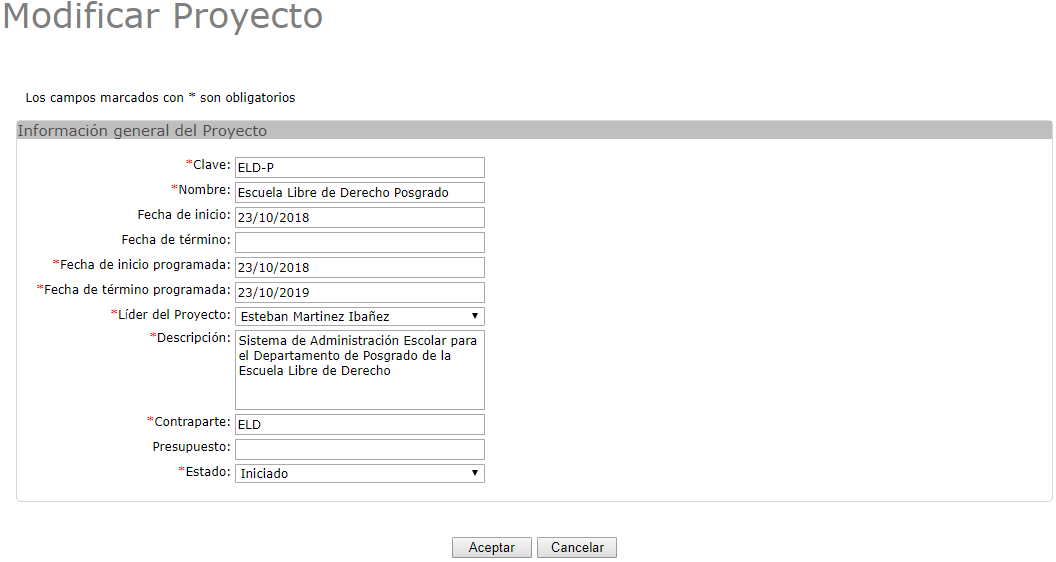
\includegraphics[scale=0.6]{roles/administrador/proyectosAdmin/gestionarproyectosAdmin/pantallas/IU2-2modificarProyecto}
					\caption{Modificar Proyecto de Administrador}
					\label{fig:modificarProyecto}
				\end{center}
			\end{figure}
		
			\item Modifique los datos solicitados por la pantalla.
			
			\item Oprima el botón \IUAceptar.
			
			\item Se mostrará el mensaje \ref{fig:proyectoModificado} en la pantalla \ref{fig:GestionarProyectosAdmin} ''Gestionar Proyectos de Administrador''.
			
			\begin{figure}[htbp!]
				\begin{center}
					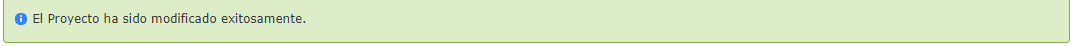
\includegraphics[scale=0.6]{roles/administrador/proyectosAdmin/gestionarproyectosAdmin/pantallas/IU2-2MSG1}
					\caption{MSG: Proyecto modificado}
					\label{fig:proyectoModificado}
				\end{center}
			\end{figure}
			\end{enumerate}